\documentclass[10pt,a4paper,twocolumn]{article}
\usepackage[margin=19mm,headheight=14pt,headsep=7mm,footskip=11mm]{geometry}
\usepackage[T1]{fontenc}
\usepackage{lmodern,microtype,amsmath,booktabs,graphicx,xcolor,fancyhdr,draftwatermark,pgfplots,hyperref}
\pgfplotsset{compat=1.18}
\definecolor{ink}{HTML}{243548}
\definecolor{teal}{HTML}{237E8A}
\definecolor{notice}{HTML}{A33D30}
\hypersetup{colorlinks=true,urlcolor=teal,pdftitle={SYNTHETIC DEMONSTRATION: Execution-strength dial},pdfauthor={Synthetic presentation example},pdfsubject={Invented data, not experimental evidence}}
\SetWatermarkText{SYNTHETIC DATA}
\SetWatermarkColor[gray]{0.94}
\SetWatermarkScale{0.40}
\pagestyle{fancy}
\fancyhf{}
\fancyhead[L]{\small\sffamily\color{notice} SYNTHETIC DEMONSTRATION}
\fancyhead[R]{\small\sffamily Invented results}
\fancyfoot[L]{\footnotesize\color{notice} Not experimental evidence}
\fancyfoot[R]{\footnotesize\thepage}
\setlength{\columnsep}{7mm}
\setlength{\parindent}{0pt}
\setlength{\parskip}{4pt}
\setlength{\emergencystretch}{2em}
\color{ink}
\begin{document}
\twocolumn[{
\begin{center}
{\Large\bfseries A Synthetic Demonstration of an\\Execution-Strength Dial}\par
\vspace{3pt}
{\normalsize Illustrative supervisor-style report, 19 October 2026}\par
\vspace{6pt}
\fcolorbox{notice}{notice!5}{\parbox{.94\textwidth}{\small\bfseries\color{notice}
All outcome counts and the plotted improvement below are invented for a demo.
They were chosen to illustrate a desirable response, not obtained from ManiGuard.
The actual pilot did not establish a safety or completion benefit.}}
\end{center}
\vspace{3pt}
\textbf{Abstract.} This presentation example explains how a compact controller around
a frozen manipulation policy could be evaluated. A hypothetical execution-strength
dial limits joint-target changes and alters feedback timing. Hand-authored counts
illustrate rising safe completion and falling violations as the dial increases.
No simulator episode, optimizer run or trained model produced these numbers.
The example demonstrates a reporting format and an intended behaviour, not an
empirical result. The original adverse pilot outcomes are retained explicitly below.
\vspace{9pt}
}]

\section{Question and system}
The research question is whether a small execution controller can improve safe task
completion around a frozen manipulation policy. Completing the requested movement
and respecting physical requirements are separate outcomes. A robot can finish while
tipping a protected object, or remain within the monitored limits while failing to finish.

The underlying policy receives camera images and robot state, then proposes a sequence
of arm and gripper commands. The execution controller may limit arm targets and request
fresh policy instructions. The policy weights remain fixed. ManiGuard's native monitor
labels violations; it does not veto or replace commands.

This system description is based on the existing implementation. The favourable
outcomes in this document are fictional and do not validate that implementation.

\section{An illustrative dial}
Let $p_t$ be a proposed arm target and $q_t$ the measured joint positions. A uniform
target limiter can scale their difference:
\[
 e_t=p_t-q_t,\qquad a_t=q_t+s_te_t,
\]
where $s_t$ is at most one and chosen so that the largest absolute joint-target
change does not exceed a declared cap. Scaling all coordinates together preserves
the direction of the joint-error vector before downstream processing. It does not
guarantee a straight hand trajectory, safe forces or upright objects.

An execution-strength dial blends the proposal and adapted target:
\[
 u_t=(1-d)p_t+d a_t,\qquad 0\le d\le1.
\]
Identity uses $d=0$; full adaptation uses $d=1$. Native action-space clipping remains
a subsequent boundary. Gripper proposals are unchanged in this simplified example.
The feedback schedule must also be specified before a real comparison.

Higher $d$ means stronger adaptation. A monotonic safety improvement would need
measurement; the dial equation alone cannot establish it.

\section{Synthetic outcomes}
The example assigns 40 fictional episodes to each setting. The four mutually
exclusive categories sum to 40 in every row. Violations comprise both unsafe
completion and unsafe unfinished episodes. Unfinished episodes comprise both safe
and unsafe unfinished episodes.

\begin{center}
\small
\textbf{Invented counts, not recorded episodes}\par\smallskip
\begin{tabular}{lrrrr}
\toprule
Setting & SC & UC & SU & UU\\
\midrule
Identity & 20 & 4 & 12 & 4 \\
Half & 27 & 2 & 9 & 2 \\
Full & 32 & 1 & 6 & 1 \\
\bottomrule
\end{tabular}

\par\smallskip
\footnotesize SC: safe complete; UC: unsafe complete;\\
SU: safe unfinished; UU: unsafe unfinished.
\end{center}

These hand-chosen counts give safe completion of 50\%, 67.5\% and 80\%, with
violations of 20\%, 10\% and 5\%. Total unfinished proportions are 40\%, 27.5\%
and 17.5\%. Thus this example illustrates the intended pattern without hiding
inactivity or unsafe completion. The pattern follows directly from how the counts
were constructed. It is not a discovery.

\begin{figure}[ht]
\centering
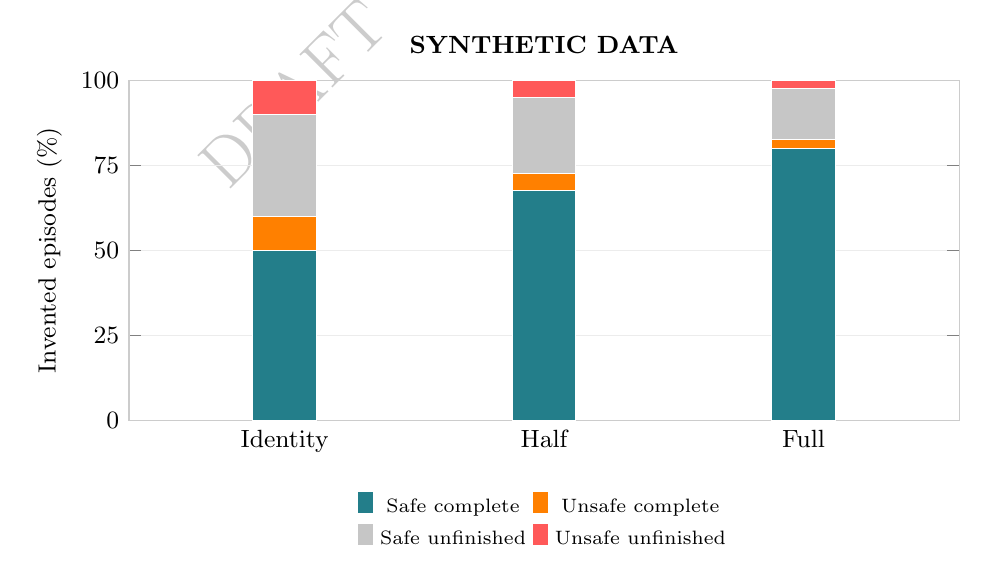
\begin{tikzpicture}
\begin{axis}[
width=\linewidth,height=5.9cm,
ybar stacked,bar width=23pt,ymin=0,ymax=100,
xtick={0,1,2},xticklabels={Identity,Half,Full},
ytick={0,25,50,75,100},ylabel={Invented episodes (\%)},
title={\small\bfseries SYNTHETIC DATA},
tick label style={font=\small},label style={font=\small},
legend style={at={(.5,-.19)},anchor=north,legend columns=2,font=\scriptsize,draw=none},
enlarge x limits=.3,ymajorgrids=true,grid style={gray!15},
axis line style={gray!40}]
\addplot[fill=teal,draw=white] coordinates {(0,50.00) (1,67.50) (2,80.00)};
\addplot[fill=orange,draw=white] coordinates {(0,10.00) (1,5.00) (2,2.50)};
\addplot[fill=gray!45,draw=white] coordinates {(0,30.00) (1,22.50) (2,15.00)};
\addplot[fill=red!65,draw=white] coordinates {(0,10.00) (1,5.00) (2,2.50)};

\legend{Safe complete,Unsafe complete,Safe unfinished,Unsafe unfinished}
\end{axis}
\end{tikzpicture}
\caption{Synthetic demonstration only. Counts were chosen by hand to show a
desirable dial response. No plotted bar represents a measured simulator outcome.}
\end{figure}

\section{Scope of the example}
No search procedure generated a finalist for this example. It therefore provides
no evidence for evolutionary advantage over random search or ordinary learning.
There are no independent optimizer seeds, new scenes, trajectories or measured costs.
The fictional denominator of 40 is a presentation choice, not an experimental allocation.

No confidence interval or significance test is attached to these invented counts.
Increasing the fictional sample size would not create empirical support.
Likewise, fewer invented violations do not establish a calibrated safety control,
real-robot safety or transfer to another manipulation task.

\section{Actual pilot outcomes}
The recorded Part 1 comparison had eight episodes per setting, not 40. Identity
achieved \textbf{5/8 safe completions and 0/8 violating episodes}; half adaptation
achieved \textbf{3/8 and 2/8}; full adaptation achieved \textbf{4/8 and 2/8}.
The selected controller did not improve that comparison. Its small denominator
limits broader conclusions but does not make the observed outcome favourable.

Part 2's adaptive refresh never requested an early query in its physical pilot.
The later direction-preserving limiter was checked on saved traces; improved
physical outcomes remain untested. Parts 3 and 4 did not establish useful prediction
prerequisites for their planned evolutionary comparisons.

These facts remain in the original supervisor draft. The synthetic data in this
document do not replace, correct or extend any experimental record.

\section{Evidence still needed}
A new study would first freeze the controller semantics, dial settings, task
partitions and evaluation rule. It would then execute all declared conditions,
preserve every attempt, and report safe completion, violations and unfinished
episodes together. Command limiting and feedback timing should be isolated so
that an improvement has an interpretable mechanism.

To attribute a benefit to evolution, compare it with matched random search,
ordinary learning and a fixed controller using the same information and accounting
for actual simulator interactions, policy queries and elapsed time. Freeze
finalists before independent evaluation and retain null or adverse outcomes.
This describes needed evidence; those comparisons were not performed for this demo.

\section{Provenance and use}
The accompanying \texttt{demo-data.json} explicitly marks every aggregate as
synthetic. A small builder validates category totals and generates the table and
chart directly from that file. No raw traces or private checkpoints are consumed.
The same folder contains the editable source and rebuild instructions.

For a live presentation, introduce the chart as: ``This is an invented example
of the behaviour we would like to demonstrate. Our actual pilot did not show it.''
Keep this qualification visible if a figure or table is copied into another medium.

\begingroup\raggedright\small
\textbf{Original evidence source:} repository file
\texttt{docs/research/reports/}\allowbreak
\texttt{maniguard-phase3-part1-gecco/}\allowbreak
\texttt{supervisor-draft.tex}, commit \texttt{54a1020}.
The original report and its recorded outcomes were left unchanged.
\par\endgroup
\end{document}
